\documentclass[11pt,twoside,a4paper]{article}
\usepackage{latexsym}
\usepackage{graphicx}
\usepackage{float}
\newcommand*\rfrac[2]{{}^{#1}\!/_{#2}}
\DeclareGraphicsExtensions{.pdf,.png}

\begin{document}
	\title{Carbon Nanotube Sensors for Synthetic Skin}
	\author{Hamish Colenso}
	\date{December 2015}
	\maketitle
	
	\begin{abstract}
		Hello World.
		Hi Hamish! :)
	\end{abstract}
	
	\newpage
	\section{Introduction}
		\subsection{Orthotic Rehabilitation}
		\subsection{Carbon Nanotubes}
		\subsection{something something something}
	\newpage
	\section{Method}
		Device creation is split into subprocesses which are described in more detail below. The basic premise of the device creation is to produce a flexible substrate, deposit contacts 			onto this substrate, deposit the sensor material onto the substrate, repeat the process, cover one device with a deformable dielectric, sandwich the two layers together and 			finally encapsulate the device in a protective outer coating. 
		\newline
		\begin{figure}[H]
			\centering
			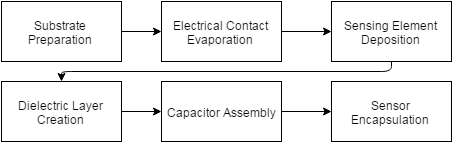
\includegraphics[scale=.8]{ProcessDiagram}
			\caption{The process for creating a capacitive sensor device}
		\end{figure}
		\subsection{Preparation}
			\begin{enumerate}
				\item Cut slides
				\item Mix PDMS 10:1 base to curing agent ratio
				\item Pour 12 ml PDMS into petri dish covered in slides
				\item Leave to set
				\item Cut individual slides away
				\item Flip PDMS over to reveal smooth surface from glass slide
			\end{enumerate}
		\subsection{Evaporation}
			\begin{enumerate}
				\item Kapton tape samples to sample holder, leave 1-2 mm for contacts on either edge of the sample
				\item Load samples into evaporate and pump down evaporator
				\item Deposit 5 nm of Cr
				\item Deposit 75 nm of Au
				\item Contacts formed bring evaporator back to room pressure to remove samples
			\end{enumerate}
		\subsection{CNT Deposition}
			\begin{enumerate}
				\item Set Hotplate to $150^oC$
				\item Mix a tiny concentration of CNTs (less than a pinch on the end of the spatula) with 10-12 ml NMP
				\item Sonicate CNTs @ $40^oC$ for 2 hours
				\item Load samples into sample holder on hotplate
				\item Set Air Pressure on Airbrush to 2 Bar
				\item Test AirBrush with some IPA
				\item Spray CNT solution using the airbrush, wait for NMP to evaporate from the sample between sprays
				\item Spray NMP:CNT solution and check conductivity of film once NMP has evaporated
			\end{enumerate}
		\subsection{Optional ILL}
		
		\subsection{Optional RIE}
		
		\subsection{Dielectric Layer}
		
		\subsection{Device Encapsulation}
		
	\newpage
	\section{Results}
		\begin{enumerate}
			\item Capacitive sensors for strain and touch applications \newline
				This should show that it is possible to both compress the sensor, that is change the dielectric thickness for a response. It also should show that it is possible to stretch 				the sensor, both compressing the dielectric thickness and decreasing the plate coverage area. The devices should be able to withstand 200\% strain and decent 					compressive forces.
			\item $ \rfrac{\Omega}{\Box} $ film characterisation \newline
				This should show that the gauge factor increases as we approach sensor destruction during stretch events. So we have a trade off between a sensor that is reliable 	
				and a sensor that provides the performance characteristics required for mobile applications.
			\item Overshoot removal and power improvements \newline
				This should show that the capacitive sensors remove overshoot when compared to resistive sensors, and that the dielectric leakage from the devices is much less					than the resistive sensors. This will indicate the sensors have improved power consumption performance for mobile applications when compared to the resistive 						devices
		\end{enumerate}
	\newpage
	\section{Evaluation}
		\subsection{Comparison to objectives for orthotic rehabilitation}
	\newpage
	\section{Conclusion}
		\subsection{Indicative results indicate the potentional for this to be applied to rehabilitation devices}
\end{document}